\documentclass[12pt,a4paper,catalan]{article}
\usepackage[utf8]{inputenc}
\usepackage{graphicx} % for images
\usepackage{booktabs} % for tables
\usepackage{fancyhdr} % for header and footers
\usepackage{titlesec}
\usepackage{hyperref} % for links 
\usepackage{minted}
\usepackage{amsmath} % for math annotations
\usepackage{todonotes}
\usepackage{enumitem}
\usepackage{amsfonts}
\usepackage{subcaption}
%\usepackage{caption}
%\usepackage{siunitx}


%Definició de noms:
\newcommand{\titleTFG}{Sistema intel·ligent de suport al tutor d'estudis}
\newcommand{\myname}{Xavier Moreno Liceras}



\setlength{\parindent}{0pt}

%Definició de colors:
\definecolor{bgcode}{rgb}{0.93, 0.93, 0.93}

%\setcounter{secnumdepth}{4}
%\setcounter{tocdepth}{4}
\titleformat{\paragraph}
{\normalfont\normalsize\bfseries}{\theparagraph}{1em}{}
\titlespacing*{\paragraph}
{0pt}{3.25ex plus 1ex minus .2ex}{1.5ex plus .2ex}

% define letters
\makeatletter
\def\iddots{\mathinner{\mkern1mu\raise\p@
\vbox{\kern7\p@\hbox{.}}\mkern2mu
\raise4\p@\hbox{.}\mkern2mu\raise7\p@\hbox{.}\mkern1mu}}
\makeatother

\pagestyle{fancy}
\fancyhf{}
\rhead{\titleTFG}
\cfoot{\thepage}
 
\hypersetup{
    unicode=true,          % non-Latin characters in Acrobat’s bookmarks
    pdftitle={\titleTFG},    % title
    pdfsubject={TFG},
    pdfauthor={\myname},     % author
    pdfproducer={\LaTeX},   % producer
    pdfcreator={\myname},   % creator of the document
    pdfkeywords={tutor} {innovació docent} {predicció} {pla d'acció tutorial}, % list of keywords
    colorlinks=true,       % false: boxed links; true: colored links
    linkcolor=blue,          % color of internal links (change box color with linkbordercolor)
    citecolor=blue,        % color of links to bibliography
    urlcolor=blue           % color of external links
}

\begin{document}

\bibstyle{plain}
\thispagestyle{empty}

\begin{titlepage}
\begin{center}
\begin{figure}[h]
\begin{center}

\includegraphics[width=6cm]{img/ub.png}
\end{center}
\end{figure}

\textbf{\LARGE Treball final de grau} \\
\vspace*{.5cm}
\textbf{\LARGE GRAU D'ENGINYERIA INFORMÀTICA } \\
\vspace*{.5cm}
\textbf{\LARGE Facultat de Matemàtiques \\ Universitat de Barcelona} \\
\vspace*{1.5cm}
\rule{\textwidth}{0.1mm}\\
\begin{Huge}
\textbf{\titleTFG} \\
\end{Huge}
\rule{\textwidth}{0.1mm}\\

\vspace{1cm}

\begin{flushright}
\textbf{\LARGE Autor: \myname}

\vspace*{2cm}

\renewcommand{\arraystretch}{1.5}
\begin{tabular}{ll}
\textbf{\Large Directora:} & \textbf{\Large Laura Igual } \\
\textbf{\Large Realitzat a:} & \textbf{\Large  Departament   } \\
 & \textbf{\Large Matemàtica Aplicada y Anàlisis} \\
\\
\textbf{\Large Barcelona,} & \textbf{\Large \today }
\end{tabular}

\end{flushright}

\end{center}
\end{titlepage}

\pagenumbering{roman}

\todo{Ha de ser redactat en primer persona del present}
\todo{Revisió de les faltes d'ortografia}


\section*{\textit{Abstract}}
\textit{Fins ara a la Facultat de Matemàtiques de la Universitat de Barcelona, cada tutor d'estudis té assignat un grup d'estudiants. Com és obvi, el tutor no pot tenir un coneixement ampli de la situació de cada alumne i és per això que aplica una serie d'accions comunes per a cadascún. Amb aquest projecte d'innovació proposem una eina de suport per al tutor d'estudis, la qual permeti ajudar al tutor a conèixer millor el perfil de cada alumne que tutoritza, amb el suport de dades estadístiques per perfil d'alumne i un recomanador que indica quant de difícil li pot arribar a costar una assignatura a un alumne.}

\section*{\textit{Resum}}
\textit{Fins ara a la Facultat de Matemàtiques de la Universitat de Barcelona, cada tutor d'estudis té assignat un grup d'estudiants. Com és obvi, el tutor no pot tenir un coneixement ampli de la situació de cada alumne i és per això que aplica una serie d'accions comunes per a cadascún. Amb aquest projecte d'innovació proposem una eina de suport per al tutor d'estudis, la qual permeti ajudar al tutor a conèixer millor el perfil de cada alumne que tutoritza, amb el suport de dades estadístiques per perfil d'alumne i un recomanador que indica quant de difícil li pot arribar a costar una assignatura a un alumne.}

\section*{\textit{Resumen}}
\textit{Hasta ahora cada tutor de estudios de la Facultad de Matemáticas de la Universidad de Barcelona tiene asignado un grupo de estudiantes. Como es obvio, el tutor no puede tener un conocimiento amplio de la situación de cada alumno y es por eso que aplica una serie de acciones comunes para cada uno. Con este proyecto de inovación docente proponemos una herramienta de soporte para al tutor de estudios, la cual permita ayudar al tutor a conocer mejor el perfil de cada alumno que tutoriza, con el soporte de datos estadísticos por cada perfil de alumno existente y un recomendador que indica lo difícil que le puede llegar a costar una asignatura a un alumno.}

\newpage 

\section*{Agraïments}

Vull agrair a ... 

\newpage
\thispagestyle{empty}
{\hypersetup{linkcolor=black}
	\tableofcontents
}
\thispagestyle{empty}
\newpage

\pagenumbering{arabic} 
\setcounter{page}{1}


\section{Introducció}
Un dels components bàsics de l'activitat docent és l'acció tutorial, la qual té com a finalitat guiar i aconsellar a l'estudiant durant la seva etapa d'estudis. Ajuda a l'estudiant a millorar el seu rendiment, a la seva orientació professional, i el més important, ajudar a prendre decissions que afavoreixin els seus estudis i la seva satisfacció. Per un altre banda tenim el pla d'acció tutorial (PAT) que tracta d'un document amb un conjunt ordenat d'accions sistemàtiques previament planificades. Una de les coses que impulsa el PAT és l'assignació d'un tutor d'estudis a un grup d'estudiants. Un tutor d'estudis, per tant té com a finalitat entre altres, acompanyar a l'alumnat durant el seu transcurs estudiantil des de l'inici del grau fins al final, aconsellant-lo per cara al món professional.
\\
\\
Ens hem trobat amb el problema que el tutor no pot tenir un control dedicat per cada alumne que tutoritza. Els pot guiar de forma genèrica, així seguint el pla d'acció tutorial. A partir de l'experiència s'ha pogut arribar a conclusions com ara que alumnes amb qualificacions moderades a primer i segon del grau d'Enginyeria Informàtica tenen problemes per afrontar certes assignatures de tercer. Ara bé, a aquest coneixement s'ha pogut obtenir a través de l'experiència, però i si estem evitant altres problemes que no s'han pogut obervar? Això ens ha fet veure que convé observar bé tots aquests successos i d'aquí ha nascut aquest projecte d'innovació docent.
\\
\\
Volem crear un sistema intel·ligent de suport al tutor d'estudis. Una eina que el tutor pogui consultar i li ajudi a prendre decissions cara a les seves tutories. Per tant de la mateixa manera que l'experiència ens ha donat coneixement al llarg del temps (com el cas explicat anteriorment), l'objectiu d'aquest projecte és obtenir coneixement a partir de les dades, i és per això que hem convertit aquest projecte en un projecte de ciència de les dades. Hem hagut de contactar amb el Vicerectorat de Política Docent, qui ens ha proporcionat les dades necessaries per realitzar aquest projecte d'innovació docent. A partir d'aquestes dades hem pogut donar perfils d'estudiants per cursos i per ensenyament, depenent de les seves notes en el grau. També hem fet un sistema de predicció que permet recomanar amb un ranking d'assignatures quines li aniran millor i quines pitjor en base a les seves notes actuals.



\newpage


\section{Descripció del problema}
\todo{change title}
\subsection{Explicar dades} 
Les dades que hem pogut adquirir són molt enriquidores, tenen la informació necesaria per fer un estudi ampli tant per als estudiants com per a l'estudi d'assignatures. A més les dades estan venen anonimitzades i per tant no podem saber de forma directe tota la informació d'un alumne. Les dades les tenim separades en diferents fitxers, les quals estan relacionades entre si mitjantçant identificadors, com ara un identificador d'alumne o el codi d'una assignatura.

\subparagraph{Registre d'alumnes}
Aquest fitxer conté per cada registre informació sobre un alumne en termes de matriculació: l'any d'inici de carrera, grau que realitza, la via amb la qual va accedir a la carrera, la nota d'accés a la Universitat, entre altres.

\subparagraph{Assignatures}
Aquí podem trobar informació de cada assignatura que existeix en els graus d'Enginyeria Informàtica i Matemàtiques: l'identificador de l'assignatura, el nom de l'assignatura, els crèdits ECTS corresponents a aquesta i el grau a la que pertanyen. A més a més, vam obtenir mitjantçant una altre font d'informació, per cada assignatura de quin curs i semestre es tractava. Aquesta dada la vam creuar amb l'anterior per ampliar la informació per assignatura.

\subparagraph{Qualificacions per alumne i per assignatura}
Per últim i més important, el fitxer que conté les qualificacions de tots els alumnes per assignatura, és a dir, per cada registre tenim: l'identificador de l'alumne que realitze l'assignatura, l'identificador de l'assignatura realitzada, la qualificació d'aquella assignatura, l'ensenyament del qual es tracta, l'any en el que es va realitzar l'assignatura i el tipus d'apunt (ordinaria, reconeixement o convalidada).

Per aquest projecte, majoritariament creuo les assignatures amb els alumnes, així quedant-me una taula on cada cel·la és la qualificació donat un alumne i una assignatura.

\newpage

\subsection{Ciència de les dades}
La ciència de les dades és el conjunt d'etapes per tal d'arribar a un resultat, en forma de coneixement, a partir d'un conjunt de dades. Aquesta aplica un conjunt de tècniques de diferents àreas, ara com matemàtiques, estadística, teoria de la informació o tecnologia de l'extracció d'informació.
\\
\\
Un projecte de ciència de les dades es separa en diverses etapes:
\begin{enumerate}
	\item \textbf{Preguntes} Què és el que volem explorar? Té sentit el que ens estem plantejant?
	\item \textbf{Adquisició de les dades} Com és la font d'obtenció de les dades? (Base de dades, \textit{Web Scraping})
	\item \textbf{Descripció} Aquesta fase abasta tres processos
	\begin{enumerate}
		\item \textbf{Neteja de dades} Com hem de netejar i separar les dades? (mostres atípiques, filtració, redució de dimensions, normalització, extracció de característiques)
		\item \textbf{Agregació} Com hem de recolectar i resumir les dades? (promig, desviació estàndard, box plots)
		\item \textbf{Enriquiment} Com podem afegir més informació a les nostres dades? (Cerca a altres fonts de dades adicionals)
	\end{enumerate}
	\item \textbf{Descobriment} Podem segmentar les nostres dades per trobar grups naturals i disgregats? (Clusterització, visualització)
	\item \textbf{Anàlisis} Com hem de modelar les nostres dades? (Com estan de relacionades cada variable?, Com podem determinar quines són les variables importants?)
	\item \textbf{Predicció} A partir de les dades que tenim, que podem predir del futur? (Regresions, clasificadors, recomanadors)
	\item \textbf{Evaluació} Com de segur estem dels nostres resultats? (Proves estadístiques, rendiment del model)
\end{enumerate}

\newpage

\subsection{Etapes del projecte}

\subsubsection{Preguntes}
La primera etapa va ser el plantejament de les preguntes que voliem resoldre. A partir de la plataforma trello, entre els participants del projecte vam plantejar preguntes, les quals entre tots decidiem amb quines preguntes ens quedariem i respondriem. Moltes de les preguntes no podíem saber si les podíem respondre fins que ens arribessin les dades, ja que depeniem totalment de la informació que contenien les dades.

\subsubsection{Adquisició}
L'adquisició de les dades va ser a partir del Vicerectorat de Política Docent. Les dades ens van arribar a través d'una fulla de càlcul. Tot i que les dades vinguessin anonimitzades i tractades pel departament corresponent, vam haver de fer una neteja de dades.

\subsubsection{Neteja de dades}
En aquesta etapa he hagut de netejar les dades per tal de poder treballar amb elles. Aquestes van ser les netejes que vaig fer:

\subparagraph{Canvi de format}
Com ja he explicat abans les dades ens van arribar en forma de fulla de càlcul, on en cada fulla havía una taula amb diferent informació. Per poder manipular-les millores des de Python, vaig haver de separar cada fulla en un fitxer amb format \textit{csv}, de tal manera que va quedar un fitxer \textit{csv} per taula.

\subparagraph{Canvi de nom de les columnes}
Per tal de poder creuar les diferents taules, els noms de les columnes havien de ser el mateix.

\subparagraph{Enriquiment de les dades}
A partir d'una font hem pogut adquirir el curs i semestre que es cursa cada assignatura, per tant el que faig és creuar aquestes dades amb les dades que tinc de cada assignatura per tal de tenir més informació per assignatura.

\subparagraph{Unió de graus}
L'any 2009 el grau en Enginyeria Informàtica de la UB tenia com a codi \textit{G1041}, però a partir de l'any 2010 el codi va passar a ser \textit{G1077}. Les assignatures eren les mateixes, tot i que tenien codis diferents també. Vam procedir a fer la unió dels \textit{G1041} amb \textit{G1077}, per tal de no perdre informació rellevant, ni considerar-la per separat.

\subparagraph{Eliminació del curs 2014, segon semestre}
Explorant les dades em vaig adonar que gent que s'havia matrículat aquest any 2014, però encara no havien acabat de cursar l'assignatura, en aquesta els hi apareixia un 0. Això feia que dintre de les notes dels alumnes haguéssin dades incoherents, per aquesta raó vam decidir eliminar totes les notes del segon semestre i de l'any 2014  que són un 10.91\% de les notes.

\todo{Elimino o no al final?}

\subparagraph{Normalitació de les notes}
Per tal d'evitar els canvis de mitja i variança en cada assignatura cursada per any, ja sigui per un canvi de professor, canvi de pla docent, diferents promocions, \ldots vam decidir normalitzar les notes per any i per assignatura aplicat una normalització d'unitat tipificada en la qual s'aplica per cada dada la següent fórmula:
$$ z = \frac{x - \mu}{\sigma}, $$

on $\mu$ és el promig per any i per assignatura, i $\sigma$ és la desviació estàndard per any i per assignatura. Amb això aconseguim mitja 0 i desviació estàndard 1.

\subsubsection{Clusterització}
Aquesta etapa era necessaria per poder respondre a una des les preguntes plantejades, i és: \textit{Hi ha diferents perfils d'alumnes?}. Per tal de  respondre a aquesta pregunta he aplicat mètodes de clusterització a partir de les notes dels alumnes diferenciats per cursos.

\subsubsection{Predicció}
La predicció, com s'ha explicat abans, és la predicció del futur a partir de les dades disponibles. En aquest cas hem volgut predir les notes que pot arribar a treure un alumne en base a les notes que ha tret en cursos anteriors.

\subsubsection{Evaluació}
Un cop construida la predicció, hem d'avaluar quant de bona és. Per això vaig agafar un 10\% de les meves dades per poder testejar i comprovar la tassa d'encerts de la predicció.

\newpage

\subsection{Preguntes plantejades} \todo{change title}
% Hi ha diferents perfils d'alumnes?
% Quina es la tassa d'abandonament per cada tipus de perfil?
% Cadascun d'aquests perfils amb quin perfil de provinença encaixa?
% Predicció de notes per fer un ranking de dificultats
\paragraph{Hi ha diferents perfils d'alumnes?}
A partir de la distribució de les notes de cada alumne per cada assignatura que ha fet, podem determinar que hi ha diferents perfils d'estudiants? Això és el que ens estem preguntant. He agafat tots els alumnes que hagin cursat totes les assignatures de primer i després amb segon, tant al grau d'Enginyeria Informàtica com al grau de Matemàtiques. La experiència ens diu que hi han alumnes bons en programació i dolents en les assignatures de matemàtiques a primer del grau d'Enginyeria Informàtica. Però per a la resta de cursos, quins perfil podem trobar? Ara que tenim les dades això ho podem saber, convertirem les dades en coneixement.

\paragraph{Quina es la tassa d'abandonament per cada tipus de perfil?}
A partir dels perfils que han sigut determinats en la pregunta anterior, quin és el percentatge d'abandonament per cadascun d'aquests. Volem saber si és cert que els alumnes cauen al perfil d'alumnes que ho suspenen tot són els que solen abandonar la carrera. Fins ara això sembla força obvi, però ho podem demostrar amb dades i corroborar-ho.

\paragraph{Cadascun d'aquests perfils amb quin perfil de provinença encaixa?}
Al llarg dels anys s'ha pogut notar que els alumnes que venen d'un Cicle Formatiu de Grau Superior (CFGS) solen ser alumnes que els hi dóna malament les assignatures relacionades amb les matemàtiquies i són força bons en programació. Ara bé, això és cert? Per això ens plantegem aquesta pregunta, a partir de perfils d'origen, volem saber amb quin cluster destí van a parar. En aquest cas hem fet els següents creuaments per cada grau:

\begin{table}[h]
\centering
\begin{tabular}{@{}cc@{}}
\toprule
{\bf Origen}               & {\bf Destí}                \\ \midrule
Via d'accés                & Perfil d'alumnes de primer \\
Perfil d'alumnes de primer & Perfil d'alumnes de segon  \\ \bottomrule
\end{tabular}
\end{table}
Els perfils d'alumnes de primer i segon són els perfils determinats a la primera pregunta, i els perfils de via d'accés que hem seleccionat han sigut els següents:
\begin{enumerate}
	\item Batxillerat (Batx)
	\item Salt d'Universitat (Uni)
\end{enumerate}

Hem obviat els alumnes provinents de cicle o ja diplomants, per la seva baixa presència. Les vies d'accés només les comprovem amb els alumnes que hagin cursat totes les assignatures de primer, sense convalidar, el que fa que no apareguin masses alumnes de cicle, ja que la majoria de cicle tenen alguna assignatura convalidada de primer. I pel que fa als alumnes ja diplomats, no hi han masses en totes les dades que tenim.

\paragraph{Predicció de notes per fer un ranking de dificultats}
A partir de les notes que ha tret un alumne en el seu passat, podem predir quines assignatures li aniran bé i malament en el futur? Bé, això és el que ens plantejem en aquesta última pregunta, volem recomanar a un alumne en quines assignatures anirà fluix per així pogui reforçar més el temari que es donarà en aquella assignatura. Recordem que la finalitat d'aquest projecte es que aquesta eina sigui un suport per al tutor, és a dir, la predicció no ens dirà el que ha de fer un alumne, aquesta decisió es delega al tutor que a partir d'aquesta eina en decidirà que fer.
\newpage

\section{Planificació}
\subsection{Tasques}
Les tasques d'aquest projecte són semblants a les etapaes d'un projecte de ciència de les dades. Les tasques són:
\begin{itemize}[leftmargin=.5in]
	\item Formació
	\item Preguntes
	\item Neteja de dades
	\item Clusterització
	\item Predicció
	\item Evaluació
	\item Documentació
\end{itemize}

Les úniques etapes noves que trobem són: la de formació, és la etapa dedicada l'aprenentatge autònom de les eines utilitzades; la de documentació, és el període de temps per tal de desenvolupar aquesta memòria.

\subsection{Diagrama de Gantt}
He construït dos diagrames de Gantt, un a partir de la planificació inicial i l'altre amb la planificació real per tal de veure les diferències.

\newpage

\begin{figure}[h]
\begin{center}
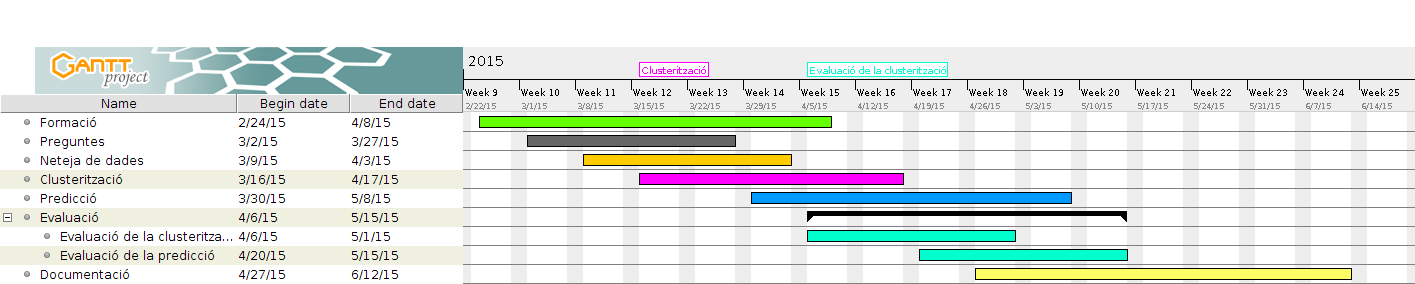
\includegraphics[width=\linewidth]{img/initialplanification.png}
\caption{Planificació inicial}
\end{center}
\end{figure}


\begin{figure}[h]
\begin{center}
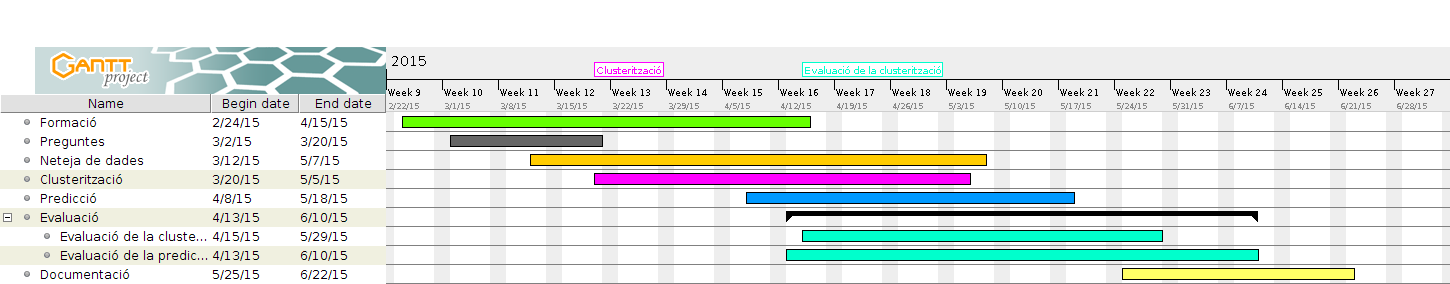
\includegraphics[width=\linewidth]{img/realplanification.png}
\caption{Planificació real}
\end{center}
\end{figure}

El Treball de fi de Grau equival a 18 crèdits ECTS, si cada crèdit equival a 25 hores, llavors tenim:

$$18\,cr\grave{e}dits \cdot \frac{25\,hores}{1\,cr\grave{e}dits} = 450\,hores$$

Per tant totes les tasques s'han de dividir en 450 hores, les hores dedicades han sigut les següents:

\begin{table}[h]
\centering

\begin{tabular}{@{}llllllll@{}}
      & \rotatebox{90}{Formació} & \rotatebox{90}{Preguntes} & \rotatebox{90}{Neteja de dades} & \rotatebox{90}{Clusterització} & \rotatebox{90}{Predicció} & \rotatebox{90}{Evaluació} & \rotatebox{90}{Documentació} \\ \midrule
Hores & 25       & 25        & 50              & 75             & 75        & 125       & 50           \\ \bottomrule
\end{tabular}
\caption{Hores de dedicació per cada tasca}
\end{table}

\newpage

\subsection{Evaluació económica}



\begin{table}[h]
\centering

\begin{tabular}{@{}llll@{}}
\toprule
                & Hores & Preu per hora (Euro) & Preu total (Euro) \\ \midrule
Formació        & 25    & 0                 & 0              \\
Preguntes       & 25    & 10                & 250            \\
Neteja de dades & 50    & 20                & 1000           \\
Clusterització  & 75    & 25                & 1875           \\
Predicció       & 75    & 25                & 1875           \\
Evaluació       & 125   & 25                & 3125           \\
Documentació    & 75    & 0                 & 0              \\ \midrule
TOTAL           & 450   &                   & 8125           \\ \bottomrule
\end{tabular}
\caption{Taula d'evaluació económica}
\end{table}

El projecte sortiria per 8125 euros, en els quals s'inclou en la etapa de Evaluació, una documentació dels resultats obtinguts i les conclusions d'aquests.

\newpage

\section{Desenvolupament del projecte}
\subsection{Eines}
\subsubsection{Eines de suport}
Aquestes són les eines de suport que m'han ajudat al llarg del treball per tal de fer més còmode la seva organització tant personal com per equip.

\paragraph{GitHub}
GitHub és una plataforma online per desenvolupar projectes software de forma col·laborativa. Aquesta plataforma utilitza un control de versions anomenat Git. La finalitat de GitHub és l'emmagatzenament massiu de projectes amb codi font obert. Per això hem optat per la utilització de GitHub, ja que que volem que el nostre codi el pogui veure tothom i que qualsevol que el necessiti per fer la seva investigació, el pogui utilitzar.

\paragraph{Bitbucket}
Bitbucket és una plataforma semblant a GitHub, però amb el servei d'un altre control de versions com Mercurial a més de Git. Bitbucket té l'advantatge de permetre crear repositoris privats de forma gratuïta. Aquesta plataforma va bé per a l'inici d'un projecte on es fan molts canvis en el codi, ja que pots tenir el codi en privat, i un cop el codi ja agafa forma es pot migrar a GitHub. Això és el que hem fet nosaltres en el projecte, començar amb Bitbucket i després passar-nos a GitHub amb el codi font obert.

\paragraph{Trello}
Per últim com eina de suport, hem fet servir Trello, una plataforma online que permet una comunicació més clara entre els membres d'un projecte. Amb Trello pots crear projectes i cada projecte conté un conjunt de llistes que s'omplen de tasques. Nosaltres hem fet servir Trello, per comunicar-nos amb la tutora i tenir present una planificació per tal d'organitzar-nos millor.

\newpage
\subsubsection{Eines de programació}
En aquesta secció trobarem amb el llenguatge de programació i conjunt de llibreries que hem treballat.

\paragraph{Python}
Python és un llenguatge d'alt nivell interpretat. Remarquen molt la fàcil lectura del seus codis, per això té una sintaxis molt semblant a un pseudocodi. Python és un llenguatge de codi obert i desenvolupat per \textit{Python Software Foundation}, una organització sense ànim de lucre. Vam escollir Python en el seu moment per dues simples raons; per ser un llenguatge de scripting i per la seves llibreries relacionades amb el tractament de dades (com \hyperlink{pandas}{Pandas}, \hyperlink{numpy}{NumPy} o \hyperlink{sklearn}{Scikit-learn}).


\hypertarget{pandas}{
	\paragraph{Pandas}
}
Pandas és una biblioteca informàtica escrita en python per a la manipulació i anàlisi de dades. Especialment va bé per al tractament de taules alhora de fer consultes, o per a l'agrupació i agrecació d'informació.

\hypertarget{numpy}{
	\paragraph{NumPy}
}
Numpy és una biblioteca informàtica de Python per operar amb vectors i matrius d'una forma més extensa a la que et permet el mateix llenguatge Python, la qual conté tot un conjunt de funcions matemàtiques d'alt nivell per treballar amb aquests vectors i matrius.

\hypertarget{sklearn}{
	\paragraph{Scikit-learn}
}
Scikit-learn és una biblioteca informàtica orientada a l'aprenentatge automàtic per a Python. Té suport per classificadors, regressors i clustering. Per aquest projecte hem fet servir clustering i regressors. En la secció de \hyperlink{tecniquesutilitzades}{Tècniques utilitzades} es detalla cada tècnica utilitzada d'aquesta biblioteca informàtica.

\paragraph{Bokeh}
Bokeh és una biblioteca informàtica per a la visualització interactiva de dades dirigida als navegadors per a la seva presentació a través d'HTML i JavaScript. Bokeh té el suport per a gràfiques específiques com diagrames de barra, box plots o time series, però a banda d'aquests gràfics pots dibuixar sobre un gràfic amb elements bàsics com cercles, línies, rectangles, entre altres.

\paragraph{Seaborn}
Per últim tenim Seaborn que també és una biblioteca informàtica per a visualitazció de dades com Bokeh, amb gràfiques molt més específiques. A més té una part de la biblioteca informàtica dedicada a les paletes de colors i la qual permet escollir un conjunt de colors afavorits per mostrar les dades.

\begin{figure}[h]
\begin{minted}
[
framesep=5mm,
baselinestretch=1.2,
bgcolor=bgcode,
fontsize=\footnotesize
]
{python}
%matplotlib inline
import seaborn as sbn
palette = sbn.color_palette("hls", 5)
sbn.palplot(palette)
\end{minted}
\begin{center}

\includegraphics[width=8cm]{img/palplot_seaborn.png}
\end{center}
\caption{Elecció d'una paleta de 5 colors}
\end{figure}


\subsubsection{Eines d'edició}
\paragraph{IPython notebook}
Ipython notebook és un editor per a l'entorn de Python. La filosofia \textit{notebook} s'emprea per tenir un codi molt més llegible i a més tenir explicacions d'allò que es programa, ja que es pot barrejar codi, la sortida del codi, markdown, HTML, entre altres. Hem optat per escollit aquest entorn d'edició ja que en un projecte de ciència de les dades s'han de veure resutats constants i poder-los comentar.

\paragraph{Texmaker}
Aquesta és una eina d'edició de \LaTeX, la qual permet poder generar informes, documents, llibres d'una forma més programàtica. A partir d'un etiquetatge estipulat podem generar documents amb un estil predefinit com el d'aquesta memòria.

\newpage
\hypertarget{tecniquesutilitzades}{
	\subsection{Tècniques utilitzades}
}
\subsubsection{Clusterització (Agrupacions)}
La clusterització és molt important en el món de les dades si el que volem es reconèixer diferents grups de ítems de les nostres dades, en el nostre cas d'alumnes. Per això, abans de veure els resultats i experiments explorats, cal entendre les diferències entre les diferents tècniques de clusterització. En aquest projecte hem fet servir dues tècniques, on l'objectiu d'elles és el mateix, desframentar les dades i trobar diferents grups d'alumnes. Aquestes dues tècniquies són K-means i MeanShift, ambdues implementades en la biblioteca informàtica de Scikit-learn. \todo{link}

\paragraph{\textit{K-means}}
\todo{Referenciar al k-means de sklearn.}
\textit{K-means} probablement és un dels algoritmes d'agrupació més conegut. Partint de $n$ elements, segmenta aquests $n$ elements en $k$ grups (entrada obligatòria de l'algoritme) on cada element pertany al grup més proper a la mitjana. L'algoritme de \textit{K-means} està descrit per la següent fórmula:
\\
\\
Tenint un conjunt d'elements $(x_1, x_2, \ldots, x_n)$ on cada elements és un vector $d$ dimensional, \textit{K-means} construeix una partició dels elements en $k$ grups, on $k \leq n$ quedant $S = \{S_1, S_2, \ldots, S_k\}$. Amb la finalitat de minimitzar la suma dels quadrats dintre de cada grup:

$$ \underset{S} {arg\,min} \sum_{i=1}^{k} \sum_{x_j \in S_i} \left\| x_j - \mu_i \right\|^2 $$

on $\mu_i$ és el centroide dels punts del conjunt $S_i$, és a dir, el punt mig.
\\
\\
Com es veu en la fòrmula, aquest algoritme depén d'una $k$, per determinar agrupacions, per tant \textit{K-means} ha de rebre com paràmetre d'entrada quants grups busquem. També podem pensar que depén del centroide $\mu_i$, però no es necessari, ja que aquest convergeix si apliquem iteracions sobre aquesta fòrmula.

\begin{figure}[h]
\centering
\missingfigure{\Huge Nice this triangle?}
\caption{Some caption}
\end{figure}

\newpage

\paragraph{\textit{Mean Shift}}
\todo{Referenciar al mean shift de sklearn.}
\textit{Mean Shift} és l'altre tècnica d'agrupació o clusterització que utilitzo en aquest projecte. L'objectiu d'aquesta tècnica és el mateix que \textit{K-means}, però el seu algoritme funciona de forma diferent, considerant l'espai de característiques com una funció de densitat de probabilitat.
\\
\\
Aquest algoritme no necessita com a entrada el número de clusters que busquem, com \textit{K-means}. Té altres paràmetres d'entrada, però són opcionals. En aquesta imatge podem veure la diferència entre \textit{K-means} i \textit{Mean Shift}.

\begin{figure}[h]
\centering
\missingfigure{\Huge Nice this triangle?}
\caption{Some caption}
\end{figure}

\newpage

\paragraph{Mètriques utilitzades}
Existeixen dos indicadors d'avaluació dels resultats de l'anàlisis de les agrupacions:
\begin{enumerate}
	\item \textbf{Supervisat} Utilitza les agrupacions reals per comparar-les amb les agrupacions donades per l'algoritme de clusterització.
	\item \textbf{No supervisat} És tot lo contrari, mesura la qualitat del propi model, basant-se en les característiques d'aquest.
\end{enumerate}

En el nostre cas, el que volem és explorar i averiguar quins perfils d'estudiants hi han, per tant hem d'utilitzar mètriques no supervisades, ja que no tenim una referència per comparar. La única mètrica no supervisada que utilitzem és la \textit{Silhouette}.

\todo{Referenciar a Silhouette de sklearn.}
\subparagraph{\textit{Silhouette}}
És una mesura no supervisada, que valora la integrat de cada node dintre d'un cluster. Per cada punt (o observació) calculem la \textit{silhouette} amb la següent fórmula:

$$ s(i) = \frac{b(i) - a(i)}{\max\{a(i),b(i)\}} $$

on:
\begin{itemize}[leftmargin=.5in]
	\item [$i$] és el punt del qual volem calcular la \textit{silhouette}.
	\item [$a(i)$] és la distància mitja als demés punts dintre del cluster de $i$.
	\item [$b(i)$] és la distància mitja als punts que no estan dintre del cluster de $i$.
\end{itemize}

Un cop tenim la \textit{silhouette} calculada per cada observació, per tenir la \textit{silhouette} del cluster, fem la mitja de totes elles.

\newpage

\subsubsection{Predicció}
La etapa de predicció és important en un projecte de data science, ja que ens permet predir el futur d'una forma estadística en base a les observacions que tenim. Però igual que la clusterització, hi han diverses tècniques, aquí explicaré quines tècniques he utilitzat per aquest projecte.

\todo{lincar la teoria de TNUI - recommenders}
\paragraph{Recomanador}
Una de les tècniques per predir dades són els recomanadors. En aquest apartat explicaré com funciona el recomanador que he montat possant-nos en context del nostre projecte. Tenint en compte les notes d'un conjunt d'alumnes, el recomanador és capaç de predir de forma estadística les notes d'un alumne en base a la resta dels altres.
\\
\\
Imaginem que tenim una matriu tal que:
$$
C = \bordermatrix{~ &         a_1   &    a_2   &   \cdots    &    a_m  \cr
                  e_1    &  c_{11}  &     ?    &   \cdots    &  c_{1m} \cr
                  e_2    &  c_{21}  &  c_{22}  &   \cdots    &    ?    \cr
                  \vdots &  \vdots  &  \vdots  &   \ddots    &  \vdots \cr
                  e_n    &    ?     &  c_{n2}  &   \cdots    &  c_{nm} \cr
                  }
$$

on:
\begin{itemize}[leftmargin=.5in]
	\item [$e_i$] és un estudiant.
	\item [$a_i$] és una assignatura.
	\item [$c_{ij}$] és la nota d'un alumne en una assignatura.
	\item [$?$] són notes no completes, perquè un alumne no ha cursat. l'assignatura.
\end{itemize}

La finalitat del nostre recomanador, és omplir les notes que apareixen amb $?$ i possar la nota més adient. Abans d'explicar com funciona, introduiré els diferents tipus de recomanadors que podem tenir:

\subparagraph{Recomanador col·laboratiu bassat en estudiant}
Prediem la nota d'un alumne en base a la semblança de l'alumne amb la resta. És a dir, si n alumne $e_i$ té unes notes semblant a un alumne $e_j$, les assignatures que no ha cursat $e_i$ podrem dir que seran semblants a les notes que ha tret $e_j$ en aquelles assignatures.

\subparagraph{Recomanador col·laboratiu bassat en assignatures}
Ara en comptes de bassar-nos en la semblança entre els estudiants, ens basem en la semblança entre una assignatura amb la resta. És a dir, si una assignatura $a_i$ segueix una distribució semblant a una assignatura $a_j$, llavors podem dir que un alumne $e_i$ treurà una nota semblant en ambdues assignatures.

\subparagraph{Recomanador híbrid}
Per últim tenim la barreja dels dos recomanadors esmentats. Aquest recomanador no s'ha fet servir en aquest projecte, però es podria fer servir si es pogués apendre quin pes assignar a cada tipus de recomanador.
\\
\\
Començaré explicant el recomanador col·laboratiu bassat en l'estudiant, el qual agafaré com a base per explicar el bassat en assignatures. Imaginem que tenim una matriu semblant a la d'abans:
\\
$$
C = \bordermatrix{~      &   a_1   & \cdots  &           a_q            & \cdots  &   a_m  \cr
                  e_1    &  c_{11} & \cdots  & \textbf{c}_{\textbf{1q}} & \cdots  &    ?   \cr
                  \vdots &  \vdots & \ddots  &     \textbf{\vdots}      & \iddots & \vdots \cr
                  e_p    &    ?    & \cdots  &       \textbf{?}         & \cdots  & c_{pm} \cr
                  \vdots &  \vdots & \iddots &       \textbf{\vdots}    & \ddots  & \vdots \cr
                  e_n    &  c_{n1} & \cdots  & \textbf{c}_{\textbf{nq}} & \cdots  & c_{nm} \cr
                  }
$$
\\

El que volem és predir la nota que té el símbol $?$ en negreta a la posició $c_{pq}$. El que necessitem és aplicar a la posició que volem predir la següent fórmula:
$$
	c_{pq} = \sum_{i=1}^n{\alpha_{e_pe_i}c_{iq}}
$$
on:
\begin{itemize}[leftmargin=.5in]
	\item [$\alpha$] és una funció de similitud, que dóna pes a $c_{a_qe_j}$.
	\item [$e_i$] és un estudiant.
	\item [$a_i$] és una assignatura.
\end{itemize}

Amb aquesta fórmula podem veure la funcionalitat d'aquest recomanador, si ens fixem, com més semblants siguin dos estudiants, més pes li donarem a la nota que ha tret un dels dos per recomanar-li a l'altre. Realment aquesta fórmula és la fórmula de mitja ponderada.

\newpage

Ara bé, si el que volem és fer un recomanador bassat en assignatures, tenim dues opcions. O bé aplicar la següent fórmula:
$$
	c_{pq} = \sum_{j=1}^n{\alpha_{a_qa_j}c_{pj}}
$$
O bé, fer la transposada de la matriu anterior i aplicar la mateixa fórmula d'abans.

\todo{link de sklearn}
\paragraph{\textit{Random Forest Regressor}}
Abans d'explicar la tècnica de \textit{Random Forest Regressor}, s'ha d'entendre el concepte d'un arbre de regressió. Un arbre de regressió és una tècnica utilitzada en aprenentatge automàtic, que es defineix com un model predictiu que mapeja observacions sobre una característica a conclusions sobre el valor objectiu d'aquesta característica. En aquestes estructures d'arbre, les fulles representen un valor real d'aquella característica i les branques les conjuccions de caracterítiques que han portat fins a la fulla.

%incrustrar: http://es.wikipedia.org/wiki/Aprendizaje_basado_en_%C3%A1rboles_de_decisi%C3%B3n#/media/File:CART_tree_titanic_survivors.png

\begin{figure}[h]
\centering
\missingfigure{\Huge Nice this triangle?}
\caption{Some caption}
\end{figure}

Bé doncs, \textit{Random Forest Regressor}, no és més que un conjunt d'arbres de regressió, on el resultat és la mitja de la sortida de cada arbre, a més per a cada arbre s'aplica un soroll aleatori a les dades sense variar en la seva distribució, això fa que es benificiï al fer la mitja. 

\newpage

\todo{link de sklearn}
\paragraph{Regressor lineal}
Un regressor lineal modelitza una recta de regressió a partir d'un núvol de punts. La recta definida, és la recta més propera que passa per tots els punts. El que busca és definir una variable depenent a partir d'un conjunt de variables, és a dir:
$$
y =\beta_0+\beta_1 x_1+\beta_2 x_2+ \cdots + \beta_n x_n + \varepsilon
$$

on $\beta_i$ són termes constants i $n$ són els conjunts d'observacions que tenim. En el cas d'una sola variable depenent, tindriem un resultat com el de la figura següent:

%http://ca.wikipedia.org/wiki/Regressi%C3%B3_lineal#/media/File:Normdist_regression.png
\begin{figure}[h]
\centering
\missingfigure{\Huge Nice this triangle?}
\caption{Some caption}
\end{figure}

\todo{link de sklearn}
\paragraph{Mètriques utilitzades}
Igual que en la secció de clusterització, per a la predicció de dades, també hem utilitzat mesures per validar les nostres prediccions. En aquest hem utilitzat tant mètriques supervisades com no supervisades.

\subparagraph{Error promig absolut (MAE)}
És una mesura supervisada que és basa en fer la mitja dels errors produïts pel predictor. Està definit per la següent fórmula:
$$ \mathrm{MAE} = \frac{1}{n}\sum_{i=1}^n \left| y_{pred_i}-y_{test_i}\right| $$

\subparagraph{Error promig quadràtic (MSE)}
Per un altre banda tenim una segona mètrica supervisada també, però aquesta mètrica penalitza els error alts, ja que la diferència es elavada al quadrat, quedaria la següent fórmula:
$$\mathrm{MSE}=\frac{1}{n}\sum_{i=1}^n(y_{pred_i}-y_{test_i})^2$$

\subparagraph{Coeficient de pearson (PCC)}
El coeficient de pearson, la utilitzem com una mètrica supervisada i la fem servir per diferencia la distribució de les notes predites amb les notes reals. El coeficient de pearson està definit per la següent fórmula:
$$\mathrm{PCC} =\left| \frac{\sum_{i=1}^n(y_{pred_i} - \bar{y}_{pred_i})(y_{test_i} - \bar{y}_{test_i})}{\sqrt{\sum_{i=1}^n(y_{pred_i} - \bar{y}_{pred_i})^2  \sum_{i=1}^n(y_{test_i} - \bar{y}_{test_i})^2}}\right|$$

\subparagraph{Desviació estàndard (std)}
Per últim també calculem la desviació estàndard per veure si els errors són més o menys dispersos. La fórmula utilitzada és la següent:

$$ \sigma = \sqrt{ \frac{1}{n} \sum_{i=1}^n (\left| y_{pred_i}-y_{test_i}\right| - \mu)^2 } $$

Totes aquestes mètriques són necessaries per evaluar cada tècnica de predicció que utilitzo. Tot i així, les tècniques més importants i que tenen més pes són l'error promig absolut i quadràtic.

\subsubsection{Reducció de dimensions}
Una de les últimes tècniques que utilitzo en aquest projecte d'innovació docent és la reducció de dimensions. És imprescindible per poder visualitzar les teves dades si tenen una dimensió major que 3. Aquestes tècniques a més permeten reduïr el cost computacional sense variar en el seu resultat. Una de les tècniques utilitzades en aquest projecte és l'anàlisis de components principals (PCA).

\todo{link de sklearn}
\paragraph{PCA}
L'anàlisis de components principals o PCA el que fa és escollir un nou sistema de coordenades a partir d'una transformació lineal on s'ordenen les variances per mida i la variança amb major mida s'escollirà com eix principal, la segona variança com a segon eix, així successivament fins obtenir la dimensionalitat escollida per argument.

\newpage

\section{Experiments i resultats}
En aquest apartat s'explicarà pas per pas els resultats obtinguts per cada pregunta plantejada. Fins ara s'han llegit tots els conceptes necessaris per poder entendre aquesta secció de la documentació. Començaré amb les preguntes relacionades amb la clusterització i acabaré amb els resultats obtinguts amb la predicció de notes.
\\
\\
Abans de començar a comentar els resultats, explicaré de quines dades parteixo per respondre cada pregunta. D'inicial tenim tota una taula on cada fila és la qualificació d'un alumne donada un assignatura, per tant en cada fila tenim informació com \textit{l'identificador d'alumne, assignatura, tipus d'apunt (convalidada, ordinaria o de reconeixement), qualificació de l'assignatura,} \ldots És a partir d'aquesta taula que fem una conversió de tal manera que en cada fila ens quedi un alumne i cada columna sigui una assignatura, construint una matriu tal que així:

$$
\bordermatrix{C &         a_1   &    a_2   &   \cdots    &    a_m  \cr
                  e_1    &  c_{11}  &  c_{12}  &   \cdots    &  c_{1m} \cr
                  e_2    &  c_{21}  &  c_{22}  &   \cdots    &  c_{2m}    \cr
                  \vdots &  \vdots  &  \vdots  &   \ddots    &  \vdots \cr
                  e_n    &  c_{n1}  &  c_{n2}  &   \cdots    &  c_{nm} \cr
                  }
$$
on:
\begin{itemize}[leftmargin=.5in]
	\item [$e_i$] és un estudiant.
	\item [$a_i$] és una assignatura.
	\item [$c_{ij}$] és la nota d'un alumne donada una assignatura.
\end{itemize}

$C$ és una matriu amb coeficients reals, $C\in M_{nxn} (\mathbb{R})$ on $0 \leq c_{ij} \leq 10$, és a dir aquesta matriu no conté cap nombre desconegut i que cada alumne $e_i$ ha cursat tot el conjunt d'assignatures $\{a_1, a_2, a_3, \ldots, a_m\}$.
\\
\\
El conjunt d'assignatures que apareixen en les columnes pot variar depenent de la pregunta que volem respondre, pot ser el conjunt d'assignatures de primer, com el conjunt de les de primer més les de segon. Però a partir d'una matriu $C$ com aquesta em basaré algunes qüestions.

\newpage

\paragraph{Hi ha diferents perfils d'alumnes?}
La resposta a aquesta pregunta és trobar diferents tipus d'estudiants en relació a la seva nota (alumnes amb notes molt bones en tot, alumnes amb males notes en certes assignatures, alumnes que suspenen, entre altres). Però volem que el nostre algoritme explori els grups que hi han.
\\
\\
Com el que busquem són alumnes amb qualificacions semblants, utilitzarem la tècnica de \textit{K-means}, ja que pot agrupar alumnes en relació a la distància de les seves notes. Però clar, \textit{K-means} té una limitació, necessita com argument el número de clusters que volem segmentar. Hem de trobar una forma de poder trobar la millor $k$.
\\
\\
La primera opció que vam pensar és aplicar \textit{K-means} amb diferents \textit{k} i per cada prova, calcular la mesura de \textit{Silhouette}. L'algoritme de \textit{K-means} rep com a paràmetre una matriu com la matriu $C$ amb els alumnes que hagin cursat totes les assignatures de primer de cada grau implantat en la Facultat de Matemàtiques de la Universitat de Barcelona. 

\begin{figure}[h]
\centering
\begin{subfigure}{.45\textwidth}
  \centering
  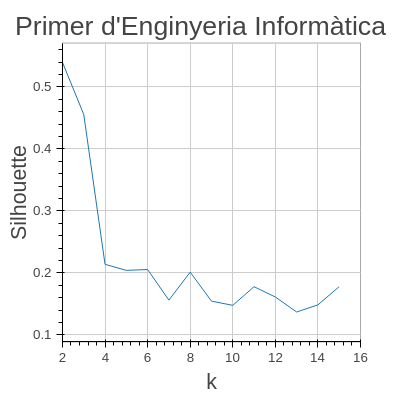
\includegraphics[width=\linewidth]{img/silhouette_primer_info.png}
  \caption{Informàtica}
\end{subfigure}
\begin{subfigure}{.45\textwidth}
  \centering
  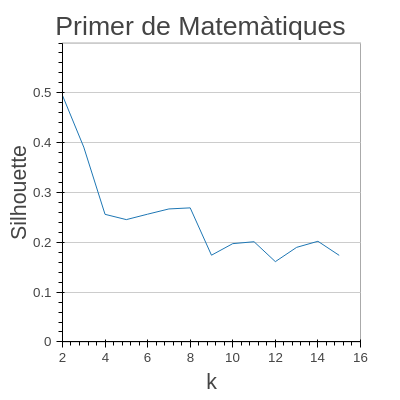
\includegraphics[width=\linewidth]{img/silhouette_primer_mates.png}
  \caption{Matemàtiques}
\end{subfigure}
\caption{Càlcul de la mesura \textit{Silhouette}}
\end{figure}

Aquest gràfic ens diu que la millor $k$ en ambdós casos és $k=2$ i la mesura de silhouette descendeix conforme augmenta el paràmetre $k$. Però clar aquest resultat no ens interesa, perquè busquem un número de clusters major que 2, encara que els clusters estiguin menys disgregats. Per tant com aquesta tècnica no ens serveix hem de buscar una altre forma per determinar quina és la millor $k$.
\\
\\
L'altre solució proposada és reduïr la dimensionalitat de les dades per tal de poder visualitzar-les en un pla dos-dimensional. Per poder fer això podem aplicar la tècnica de PCA per reduïr de 10 dimensions a 2. Un cop visualitzem cada estudiant en un espai 2D, podem aplicar un algoritme d'agrupació com \textit{Mean Shift} per veure quants clusters hi han i poder determinar una $k$ per cada curs.

\begin{figure}[h]
\centering
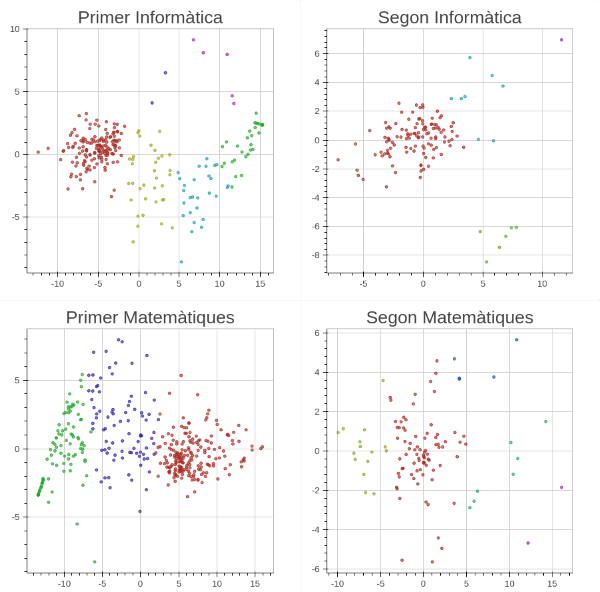
\includegraphics[width=\linewidth]{img/pca_info_mates.png}
\caption{Mean Shift després d'aplicar PCA}
\end{figure}

\newpage

Ara es poden distingir millor el número de clusters o agrupacions que trobem per cada curs.

\subparagraph{Primer d'enginyeria Informàtica}
Ens separa tot el conjunt de punts en 6 agrupacions (\textit{vermell, beix, blau claret, verd, lila i blau fosc}), però el grup \textit{blau fosc i lila} són un grup tan reduït i separat de la resta que el podriem comptar com un sol cluster. $k=5$

\subparagraph{Segon d'Enginyeria Informàtica}
Per a aquest curs ens separa als estudiants en 4 grups, i podem veure que els clusters estan força disgregats entre ells i no fa falta unificar cap.  $k=4$

\subparagraph{Primer de Matemàtiques} 
Per a primer del grau de Matemàtiques ens separa les observacions en 3 clusters. Com no es veu cap anomalia, a part de la petita separació dels petits punts verds, podem considerar els tres clusters.  $k=3$

\subparagraph{Segon de Matemàtiques}
Aquest és el curs que m'ha donat més problemes, perquè té els punts més distanciats entre ells i això fa que no es pogui interpretar el número de clusters per aplicar \textit{K-means}. Més endavant veurem que el número de clusters òptim és 3, ja que amb 4 ens dóna dos clusters molt semblants, els quals es poden unificar. $k=3$
\\
\\
Ara que ja tenim el valor de $k$ adeqüat per cada curs, podem aplicar la tècnica de \textit{K-means}. S'ha utilitzat una combinació de colors adequada per cada perfil.

\begin{figure}[h]
\centering
\begin{subfigure}{.2\textwidth}
  \centering
  
\includegraphics[width=\linewidth]{img/aprovats.png}
  \caption{Aprovats}
\end{subfigure}
\begin{subfigure}{.2\textwidth}
  \centering
  
\includegraphics[width=\linewidth]{img/bonesnotes.png}
  \caption{Bones notes}
\end{subfigure}
\begin{subfigure}{.2\textwidth}
  \centering
  
\includegraphics[width=\linewidth]{img/suspesos.png}
  \caption{Suspesos}
\end{subfigure}
\begin{subfigure}{.2\textwidth}
  \centering
  
\includegraphics[width=\linewidth]{img/altresperfils.png}
  \caption{Altres}
\end{subfigure}
\caption{Categoria de colors utilitzada per representar els perfils d'estudiants}
\end{figure}

\newpage

Començarem comentant els resultats obtinguts amb el curs de primer d'Enginyeria Informàtica on hem dit que aplicariem \textit{K-means} amb $k=5$.

\todo{retocar la imatge, per treure el quadrat gris}
\begin{figure}[h]
\centering
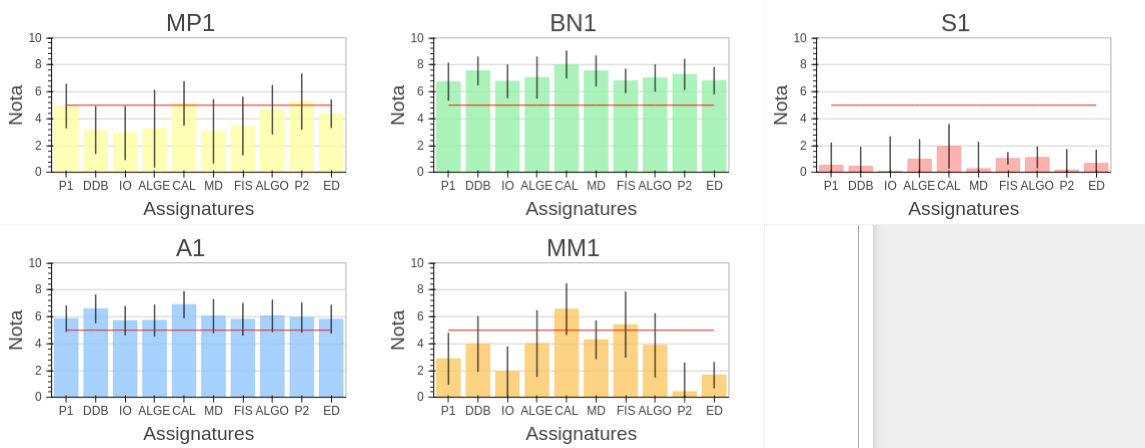
\includegraphics[width=\linewidth]{img/perfils_primer_info.png}
\caption{Perfils d'alumnes de primer d'Enginyeria Informàtica}
\end{figure}

\begin{figure}[h]
\centering
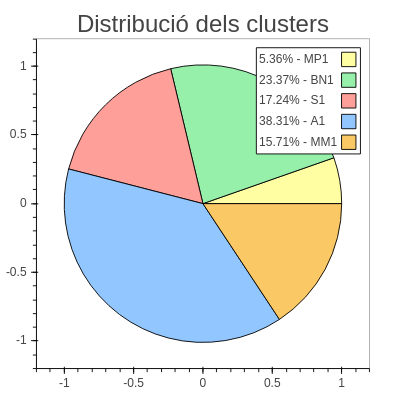
\includegraphics[width=.55\linewidth]{img/perfils_primer_info_pastilla.png}
\caption{Percentatges de cada agrupació}
\end{figure}

Primer explicaré que és el que veiem en aquests gràfics i així poder interpretar els demés. Cada gràfic són els diferents perfils d'estudiants que ha trobat la tècnica de \textit{K-means}. En cadascun d'ells trobem com a títol l'etiqueta assignada a aquell perfil i el color de cadascún depén de la categoria explicada abans. En l'eix d'abscisses es veuen les assignatures (en aquest cas les de primer d'Enginyeria Informàtica), i en l'eix d'ordenades tenim la mitja de cada assignatura (longitud de la barra). Per últim les línees negres determinen la desviació estàndard de la distribució de cada assignatura i la línea vermella és una marca per identificar l'alçada de l'aprovat.

\subparagraph{MP1 - Millors en programació de primer d'Informàtica} 
Aquest perfil encaixa amb els alumnes que tenen millores notes en les assignatures de programació que en les de matemàtiques. La distribució d'aquest és molt dispersa, això ho podem veure per la llargada de la barra negra (desviació estàndard). També és, perquè la mostra és petita, representa el 5.36\% de la mostra total.

\subparagraph{BN1 - Bones notes de primer d'Informàtica}
Aquest perfil correspon als alumnes que tenen bones notes en totes les assignatures de primer i com podem veure en el gràfic de pastilla, representen un 23.37\% del total, sent el segon perfil més abundant. Podem veure ara que la mostra és més gran, la desviació estàndard és menor, és a dir, aquest perfil és força estable, tots els estudiants que hi pertanyent es distancien amb una qualificació promig d'1.5 aproximadament.

\subparagraph{S1 - Suspesos de primer d'Informàtica}
Com podem veure, aquest perfil són els estudiants que suspenen la majoria d'assignatures. A primeres podem pensar que són els que solen deixar la carrera i és això el que anem a respondre en la següent pregunta plantejada. També podem veure que són un 17.2 \% del total d'alumnes que han cursat les assignatures de primer, no són un percentatge baix.

\subparagraph{A1 - Aprovats de primer d'Informàtica}
Són la major part dels alumnes, amb un 38.31\% del total, i són els alumnes que de mitja treuen entre 5 i 7. Igual que passa amb el cluster \textit{BN1}, la desviació estàndard de cada assignatura és força baixa, i això fa que el cluster sigui consistent.

\subparagraph{MM1 - Millors en matemàtiques de primer d'Informàtica}
Aquest perfil igual que \textit{MP1}, és bastant inestable, ja que tenen una desviació estàndard alta, és a dir, hi ha una diversitat de notes elavada, no es concentren tots els alumnes a tenir la mateixa nota. Tot i que siguin dispersos, són un 15.71 \% del total, un percentatge forç alt.
\\
\\
Fent un anàlisis general de les gràfiques, podem veure que en l'assignatura \textit{Estructura de Dades} (ED) presenta sempre una desviació més petita que la resta d'assignatures en cada perfil, és a dir, que les notes en concentren més en la mitja marcada. Per un altre banda també es pot veure que en tots els perfil, sense mirar la qualificació corresponent, la nota més alta en els 6 perfils és de l'assignatura de \textit{Càlcul} (CAL).
\\
\\
Seguint amb l'anàlisis podem veure també els perfils de tots els alumnes que hagin cursat totes les assignatures de segon, on he aplicat \textit{K-means} amb $k=4$.

\begin{figure}[h]
\centering
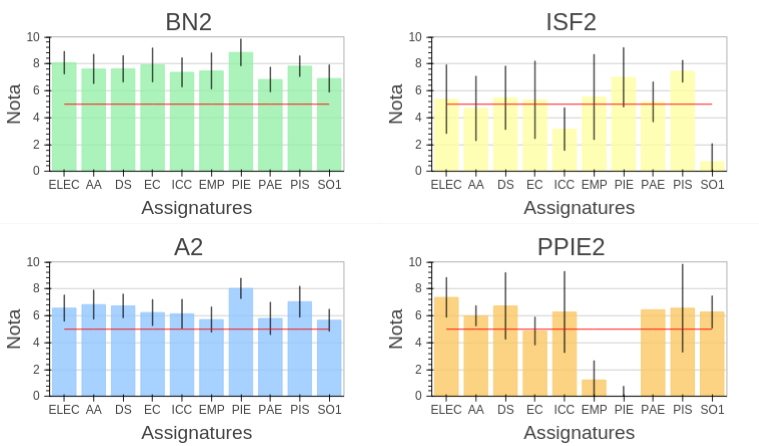
\includegraphics[width=.9\linewidth]{img/perfils_segon_info.png}
\caption{Perfils d'alumnes de segon d'Enginyeria Informàtica}
\end{figure}

\begin{figure}[h]
\centering
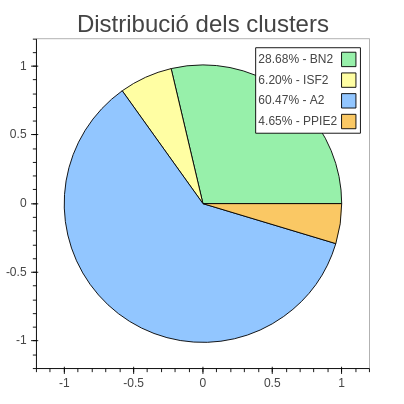
\includegraphics[width=.4\linewidth]{img/perfils_segon_info_pastilla.png}
\caption{Percentatges de cada agrupació}
\end{figure}

\subparagraph{BN2 - Bones notes de segon d'Informàtica}
Aquest és un perfil força semblant a \textit{BN1}, és per això que ens plantejem la pregunta: \textit{Cadascun d'aquests perfils amb quin perfil de provinença encaixa?}, és a dir, és cert que els que tenen bones notes a primer, solen ser els que treuen bones notes a segon, el que anomenem conservació de clusters. De tots els alumnes que han cursat segon un 28.68\% pertanyen a aquest cluster, més d'un quart de la mostra.

\subparagraph{ISF2 - ICC i SO1 fluixes}
Aquest perfil encara que sigui minoritari, amb un 6.2\% del total, és força curiós, ja que són alumnes que tenen \textit{Introducció a la Computació Científica} (ICC) i \textit{Sistemes operatius I} (SO1) amb notes més baixes que la resta. També s'ha de dir que tot i que les mitjes siguin més petites, les desviacions estàndards són molt altes, el que fa que les notes dels alumnes siguin més diverses i no segueixin exactament la distribució de mitjes de cada perfil.

\subparagraph{A2 - Aprovats de segon d'Informàtica}
Aquest perfil és semblant al perfil \textit{A1}, pertany als alumnes que tenen notes entre 5 i 7. Són el 60.47\% del total d'alumnes que han cursat les assignatures de segon.

\subparagraph{PPIE2 - Problemes amb PIE i Empresa}
Aquest és el perfil amb un percentatge més petit de població, un 4.65\%. És un perfil força dispers, ja que les desviacions estàndar són altes, i això es pot veure en assignatures com PIS o ICC. A més és curiós perquè és un grup que apareixen amb \textit{Empresa} (EMP) i \textit{Probabilitat i estadística} (PIE) suspeses, però no he trobat un perquè a aquest fenòmen.
\\
\\
Ens podem fixar que la distribució de mitjes del perfil \textit{BN2} i \textit{A2}, és força semblant, només que \textit{BN2} té les mitjes més altes.
\\
\\
Deixant enrere al grau d'Enginyeria Informàtica, em poso a analitzar als estudiants del grau en matemàtiques. Comencem amb els alumnes de primer, els quals els segmentem en 3 agrupacions ($k=3$).

\newpage

\begin{figure}[h]
\centering
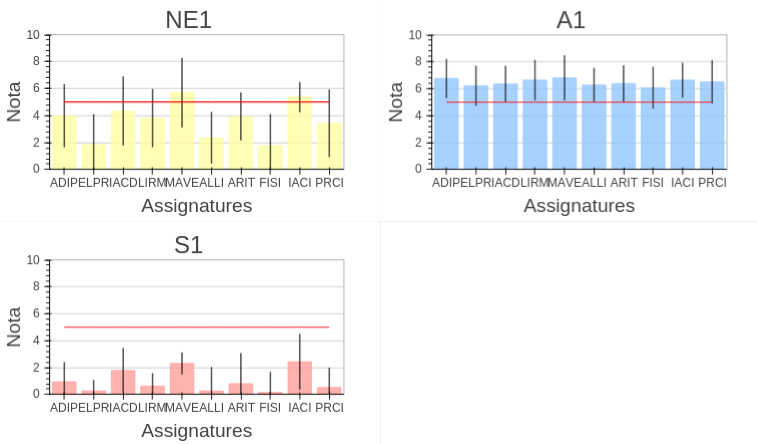
\includegraphics[width=.9\linewidth]{img/perfils_primer_mates.png}
\caption{Perfils d'alumnes de primer de Matemàtiques}
\end{figure}

\begin{figure}[h]
\centering
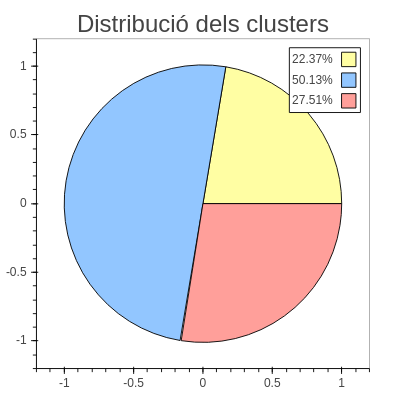
\includegraphics[width=.4\linewidth]{img/perfils_primer_mates_pastilla.png}
\caption{Percentatges de cada agrupació}
\end{figure}

\subparagraph{NE1 - No estables de primer de Matemàtiques}
Podem veure que aquest cluster té les mostres molt distanciades, per les desviacions estàndards que presenta. Aquest perfil l'he clasificat com \textit{No estables de primer}, ja que són alumnes que amb prou feines poden aprovar certes assignatures. Conformen un 22.37\% del total d'alumnes.

\subparagraph{A1 - Aprovats de primer de Matemàtiques}
Aquest perfil pertany als estudiants que tenen totes les assignatures aprovades  de mitja i són els que formen la major part del total, amb un 50.13\%.

\subparagraph{S1 - Suspesos de primer de Matemàtiques}
Per últim, i sense faltar, tenim els alumnes que de mitja suspenen totes les assignatures. Conformen un 27.51\% del total d'estudiants.
\\
\\
Els resultats són força esperats per aquest curs, tenim els que ho aproven tot i els que ho suspenen tot, i per un altre banda tenim la resta que no pertanyen ni a un ni a l'altre.
\\
\\
Per últim tenim als alumnes de segon de Matemàtiques, on no s'observa res interessant com tenim als perfils de Informàtica.

\begin{figure}[h]
\centering
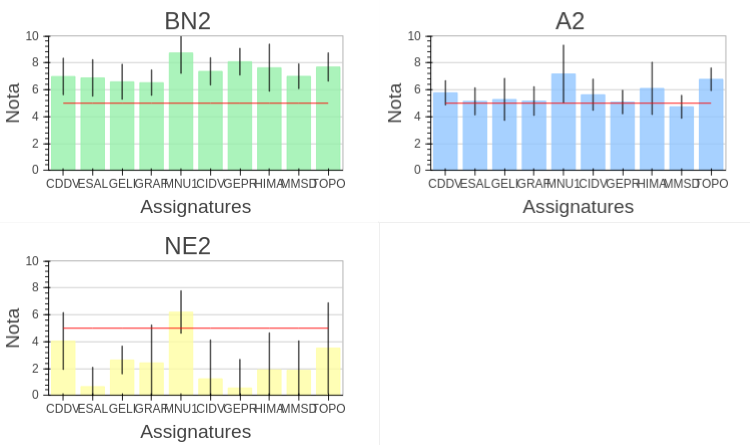
\includegraphics[width=.85\linewidth]{img/perfils_segon_mates.png}
\caption{Perfils d'alumnes de segon de Matemàtiques}
\end{figure}

\begin{figure}[h]
\centering
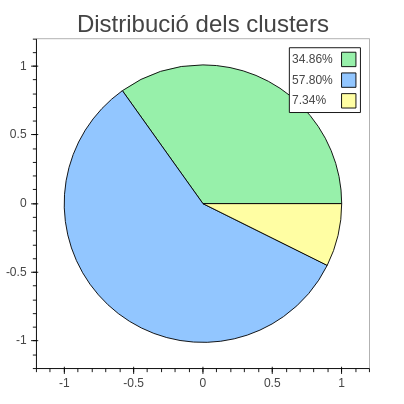
\includegraphics[width=.4\linewidth]{img/perfils_segon_mates_pastilla.png}
\caption{Percentatges de cada agrupació}
\end{figure}

\newpage

\subparagraph{BN2 - Bones notes de segon de Matemàtiques}
Torna a aparèixer aquest tipus de perfils, alumnes amb mitjes de qualificacions altes. Tot i així, és sorprenent el percentatge d'alumnes que pertanyen a aquest cluster, un 34.86\%.

\subparagraph{A2 - Aprovats de segon de Matemàtiques}
Per un altre banda tornem a tenir els alumnes amb qualificacions en el rang d'aprovat, tot i que la majoria freguen la línea de l'aprovat, com és en tots els casos, aquest és el perfil més abundant, amb un 57.80\%.

\subparagraph{NE2 - No estables de segon de Matemàtiques}
Igual que a primer del grau de Matemàtiques tenim el perfil de \textit{No estables}, aquí el tornem a tenir, tot i que aquest perfil només té aprovada per mitja una assignatura, \textit{Mètodes numèrics I} (MNU1). Pertanyen al 7.34\% del total.
\\
\\
En aquest curs tenim un efecte semblant a primer d'Enginyeria Informàtica amb l'assignatura de \textit{Càlcul}, hi ha una assignatura que en tots els perfils té la mitja més alta, \textit{Mètodes numèrics I} (MNU1).

\newpage

\paragraph{Quina es la tassa d'abandonament per cada tipus de perfil?}
És cert que els que suspenen abandonen la carrera? Ara ho podrem demostrar amb dades. Ens centrarem en la tassa d'abandonament dels alumnes que cursen primer, tant d'Enginyeria Informàtica com el grau de Matemàtiques. Tornaré a mostrar els perfils per poder contrastar cada perfil amb la seva tassa d'abandonament.

\begin{figure}[h]
\centering
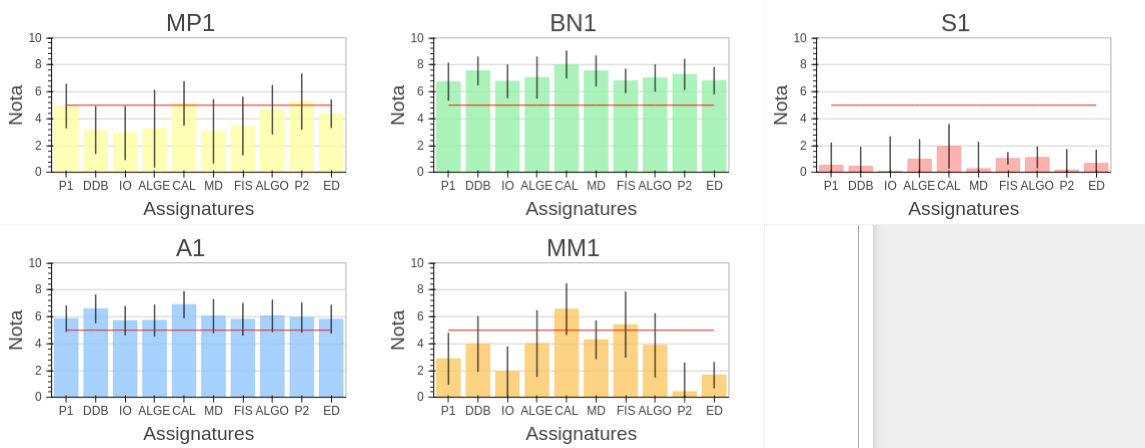
\includegraphics[width=\linewidth]{img/perfils_primer_info.png}
\caption{Perfils d'alumnes de primer d'Enginyeria Informàtica}
\end{figure}

\begin{figure}[h]
\centering
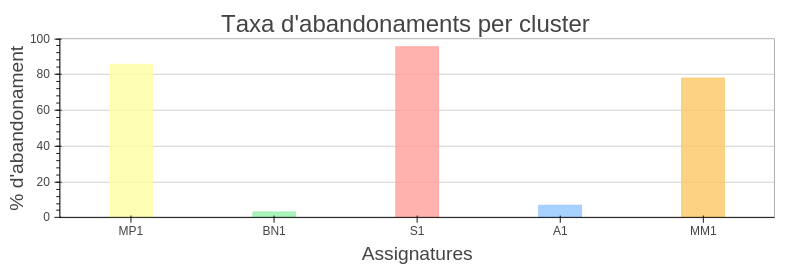
\includegraphics[width=\linewidth]{img/abandonaments_primer_info.png}
\caption{Tassa d'abandonaments per perfil}
\end{figure}

Com era d'esperar, els alumnes que amb més probabilitat deixen la carrera són els que suspenen, seguits d'estudiants que no tenen unes notes massa estables. És a dir, que la majoria que passen a segon pertanyen al cluster \textit{BN1} i \textit{A1}. Però si ens fixem una mica en el gràfic d'abandonaments, els perfils d'aprovats i de bones notes, hi ha un petit percentatge indicat que diu que abandonen la carrera. Bé, en les dades que tenim, no tenim un camp que ens indiqui si un alumne ha abandonat la carrera o no, ja que no ho tenen registrat, suposo perquè potser pot tornar un altre any l'estudiant. Com ho hem fet llavors? Hem agafat per cada perfil tot el conjunt d'alumnes d'aquell perfil i s'ha comprovat per cadascún d'ell si té assignatures matriculades a l'any següent. Però clar, hi han alumnes del darrer any que s'han de matriculat per l'any vinent encara (i no apareixen matriculats a l'any següent), per això hi ha un petit marge d'error i els clusters \textit{BN1} i \textit{A1} aparèixen amb una mínima tassa d'abandonaments. 

\begin{figure}[h]
\centering
\missingfigure{\Huge Imatge de diagrama de ben, demostrant un alumne d'abandoanet i l'altre no}
\caption{Some caption}
\end{figure}

Ara, per altre banda tenim el curs de primer de Matemàtiques, on apliquem els mateix algoritme explicat en el paràgraf anterior. També trovem un petit marge d'error en els perfils que ho aproven tot.

\begin{figure}[h]
\centering
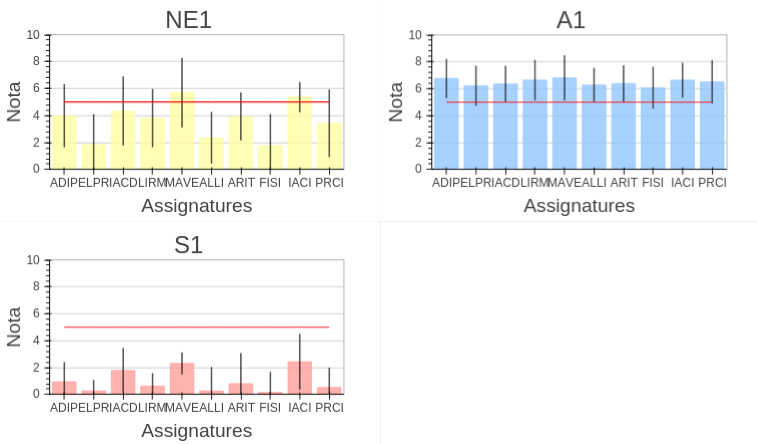
\includegraphics[width=\linewidth]{img/perfils_primer_mates.png}
\caption{Perfils d'alumnes de primer d'Enginyeria Informàtica}
\end{figure}

\begin{figure}[h]
\centering
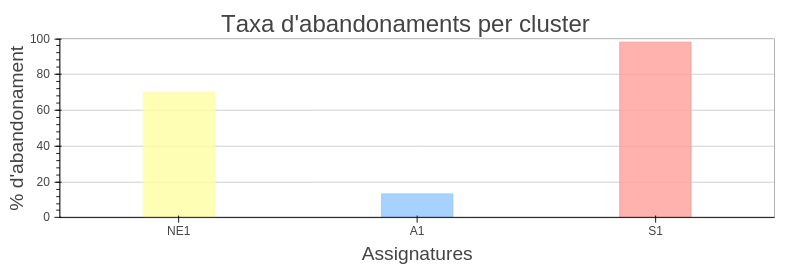
\includegraphics[width=\linewidth]{img/abandonaments_primer_mates.png}
\caption{Tassa d'abandonaments per perfil}
\end{figure}

Igual que en Enginyeria Informàtica, ens trobem que la major tassa d'abandonament es troba en els alumnes que suspenen per mitja totes les assignatures. Seguidament els hi segueixen els estudiants que no tenen unes notes massa regulars i com s'ha comentat anteriorment, els alumnes que estan classificats com \textit{Aprovats}, també surten amb una petita tassa d'abandonament.

\newpage

\paragraph{Cadascun d'aquests perfils amb quin perfil de provinença encaixa?}
El que es vol mirar en aquesta pregunta és la conservació de clusters, per exemple, els estudiants que treuen bones notes a primer, segueixen treien bones notes a segon? O, de quina via d'accés solen provenir els estudiants de primer de matemàtiques? 
\\
\\
Començarem, com hem fet anteriorment, amb els estudiants que han cursat primer d'Enginyeria Informàtica. Com s'ha explicat en la secció de preguntes plantejades, contrastem primer d'Enginyeria Informàtica amb les vies d'accés: Batxillerat i salt d'Universitat.

\todo{Canviar els colors de la gràfica}
\begin{figure}[h]
\centering
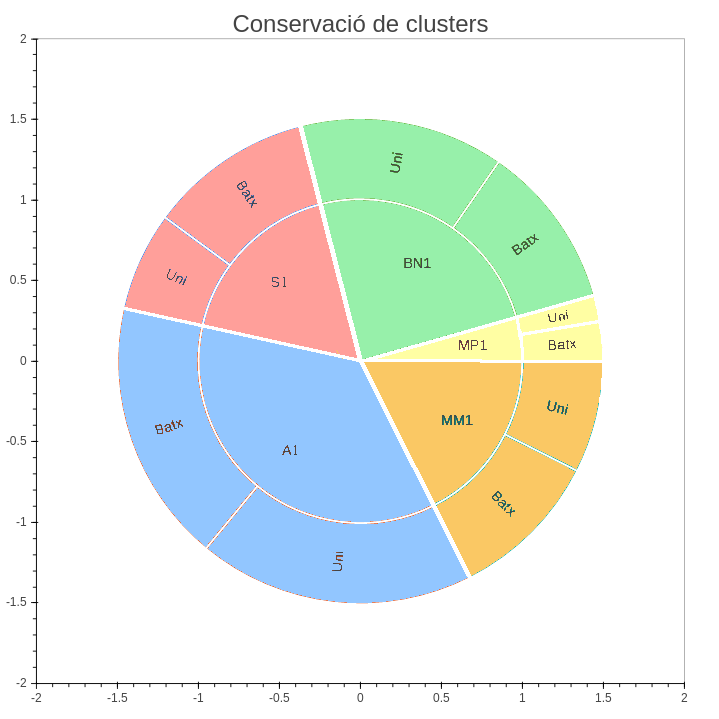
\includegraphics[width=.6\linewidth]{img/conservacio_clusters_primer_info.png}
\caption{Conservació de clusters dels alumnes de primer d'Informàtica}
\end{figure}

\todo{Possar referència a la figura anterior}
En l'interior del cercle, podem veure el mateix gràfic de pastilla que s'ha vist anteriorment dels perfils dels estudiants de primer d'Enginyeria Informàtica (AQUÍ). Per sobre de cada perfil es veu en quantitat d'on venen els alumnes del perfil. 
\\
\\
\todo{Possar referencia a la figura anterior}
Es pot veure com en tots els perfils, venen meitat de Batxillerat i meitat de Salt d'Universitat aproximadament. Es pot distingir que els estudiants classificats com \textit{Suspesos} solen venir més de Batxillerat que no pas d'una altre Universitat, tot i que la diferència és petita. Com s'ha vist en la gràfica d'abandonament (AQUÍ), els alumnes que passen amb més abundancia a segon són els classificats com \textit{A1} i \textit{BN1}, per tant procedim a eliminar a la resta, ja que són minoria, i així més llegible la següent gràfica.

\begin{figure}[h]
\centering
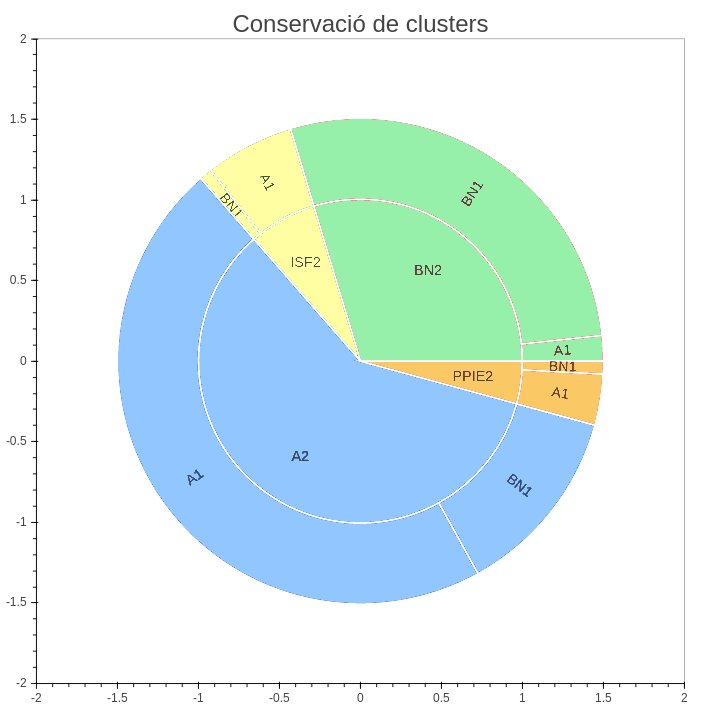
\includegraphics[width=.6\linewidth]{img/conservacio_clusters_segon_info.png}
\caption{Conservació de clusters dels alumnes de primer d'Informàtica}
\end{figure}

Ara és veu amb més claredat el significat d'un gràfic com aquest, ja que podem veure com els que solen treure bones notes a primer dEnginyeria Informàtica, solen treure bones notes a segon també, i els que classificaven com \textit{Aprovats de primer}, solen parar a \textit{Aprovats de segon}. També podem veure com un petit percentatge d'alumnes que treuen notes a primer, passen a treure notes més baixes a segon, igual que alumnes etiquetats com \textit{Aprovats de primer} amb una petit quanitat paren a perfils inestables com \textit{ISF2} o \textit{PPIE2}.

\newpage

Per últim es veurà la provinença dels estudiants de primer del grau de Matemàtiques, on també es pot veure una tendencia.

\begin{figure}[h]
\centering
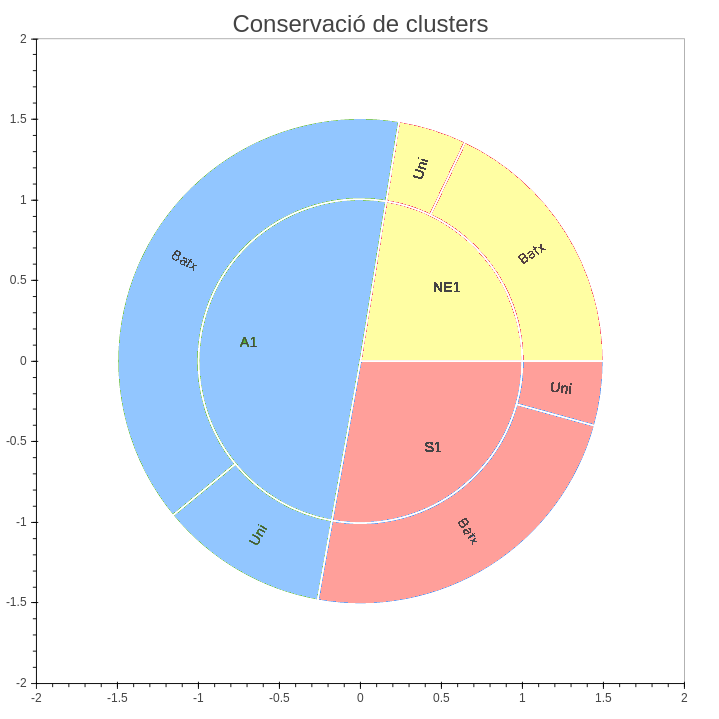
\includegraphics[width=.6\linewidth]{img/conservacio_clusters_primer_mates.png}
\caption{Conservació de clusters dels alumnes de primer d'Informàtica}
\end{figure}

En aquesta gràfica es veu amb claredat que la major part d'estudiants que han cursat primer del grau de Matemàtiques, venen de Batxillerat. 

Una de les raons per les quals vam plantejar aquesta pregunta, era per saber si podiem determinar un perfil d'estudiant al grau a partir de la via d'accés d'aquest. Malauradament no s'ha trobat cap correlació com aquesta, però s'han pogut veure resultats molt coherents i que no esperavem trobar.

\newpage

\paragraph{Predicció de notes per fer un ranking de dificultats}


\todo{No fer cas a les taules encara}
\begin{table}[h]
\centering
\begin{tabular}{@{}llll@{}}
\toprule
\textit{\textbf{Algoritme$\setminus$Mètriques}}   & \textbf{MAE} & \textbf{MSE} & \textbf{PCC} \\ \midrule
\textbf{Recomanador col·laboratiu}      & 1.231        & 2.997        & 0.335        \\
\textbf{Recomanador basat en contingut} & 1.197        & 2.905        & 0.403        \\
\textbf{Random Forest Regressor}        & 1.134        & 2.584        & 0.490        \\
\textbf{Linear Regressor}               & 1.175        & 2.720        & 0.462        \\ \bottomrule
\end{tabular}
\caption{Dades no normalitzades}
\end{table}

\begin{table}[h]
\centering
\begin{tabular}{@{}llll@{}}
\toprule
\textit{\textbf{Mètriques/Algoritme}}   & \textbf{MAE} & \textbf{MSE} & \textbf{PCC} \\ \midrule
\textbf{Recomanador col·laboratiu}      & 0.558        & 0.669        & 0.069        \\
\textbf{Recomanador basat en contingut} & 0.531        & 0.660        & 0.358        \\
\textbf{Random Forest Regressor}        & 0.509        & 0.565        & 0.393        \\
\textbf{Linear Regressor}               & 0.538        & 0.648        & 0.462        \\ \bottomrule
\end{tabular}
\caption{Dades normalitzades}
\end{table}

% Preguntes:
%   - Hi ha perfils d'estudiants basats en les notes?
%   - Un dels clusters correspon als alumnes que abandonen?
%   - Quin perfil d'entrada té cada cluster?
%   - Ranking de dificultat de les assignatures que ha de fer (que ha matriculat) un alumne
\newpage
\section{Conclusions i treball futur}
\newpage
\section{Bibliografia}
\end{document}